\documentclass[12pt]{article}
\usepackage[utf8]{inputenc}
\usepackage{float}
\usepackage{amsmath}
\usepackage[strict]{changepage}
\hbadness=10000

\usepackage[hmargin=3cm,vmargin=6.0cm]{geometry}
%\topmargin=0cm
\topmargin=-2cm
\addtolength{\textheight}{6.5cm}
\addtolength{\textwidth}{2.0cm}
%\setlength{\leftmargin}{-5cm}
\setlength{\oddsidemargin}{0.0cm}
\setlength{\evensidemargin}{0.0cm}

\newcommand{\HRule}{\rule{\linewidth}{1mm}}

%misc libraries goes here
\usepackage{tabularx}
\usepackage{tikz}
\usetikzlibrary{positioning}
\renewcommand\tabularxcolumn[1]{m{#1}}
\newcolumntype{M}{>{\centering\arraybackslash}m{1.15cm}}
\newcommand\tikzmark[2]{%
\tikz[remember picture,baseline] \node[inner sep=2pt,outer sep=0] (#1){#2};%
}

\newcommand\link[2]{%
\begin{tikzpicture}[remember picture, overlay, >=stealth, shift={(0,0)}]
  \draw[->] (#1) to (#2);
\end{tikzpicture}%
}
\begin{document}

\noindent
\HRule \\[3mm]
\begin{flushright}

                                         \LARGE \textbf{CENG 465}  \\[4mm]
                                         \Large Introduction to Bioinformatics \\[4mm]
                                        \normalsize      Spring '2019-2020 \\
                                           \Large   Assignment 2 \\
                    \normalsize Deadline: April 5, 23:59 \\
                    \normalsize Submission: via ODTUCLASS
\end{flushright}
\HRule

\section*{Student Information }
Full Name : Yasin Fatih ALPUL \\
Id Number :  2098739 \\

\section*{Part A}
Below are the state transitions for the $8$ sequences.
\begin{align*}
    1 : \text{Begin} & \rightarrow I_0 \rightarrow I_0 \rightarrow D_1 \rightarrow I_1 \rightarrow M_2 \rightarrow M_3  \rightarrow M_4\rightarrow I_4 \rightarrow \text{End}\\
    2 : \text{Begin} & \rightarrow I_0 \rightarrow I_0 \rightarrow M_1\rightarrow I_1 \rightarrow M_2 \rightarrow M_3  \rightarrow M_4\rightarrow I_4 \rightarrow I_4 \rightarrow\text{End}\\
    3 : \text{Begin} & \rightarrow I_0 \rightarrow M_1\rightarrow I_1 \rightarrow M_2 \rightarrow I_2 \rightarrow M_3  \rightarrow M_4\rightarrow \text{End}\\
    4 : \text{Begin} & \rightarrow I_0 \rightarrow I_0 \rightarrow M_1\rightarrow M_2 \rightarrow D_3 \rightarrow M_4\rightarrow I_4 \rightarrow I_4 \rightarrow I_4 \rightarrow\text{End}\\
    5 : \text{Begin} & \rightarrow I_0 \rightarrow D_1 \rightarrow I_1 \rightarrow M_2 \rightarrow M_3  \rightarrow M_4 \rightarrow \text{End}\\
    6 : \text{Begin} & \rightarrow I_0 \rightarrow I_0 \rightarrow M_1\rightarrow M_2 \rightarrow I_2 \rightarrow M_3  \rightarrow M_4\rightarrow I_4 \rightarrow I_4 \rightarrow\text{End}\\
    7 : \text{Begin} & \rightarrow I_0 \rightarrow I_0 \rightarrow M_1\rightarrow M_2 \rightarrow I_2\rightarrow M_3  \rightarrow M_4\rightarrow \text{End}\\
    8 : \text{Begin} & \rightarrow I_0 \rightarrow I_0 \rightarrow M_1\rightarrow M_2 \rightarrow M_3  \rightarrow D_4\rightarrow I_4 \rightarrow\text{End}\\
\end{align*}
By computing the frequencies of state transitions, we can create the following profile Hidden Markov Model. Note that the computations were conducted as finding the number of transitions from a state and finding the number of transitions to each of other states. For example, we have $14$ transitions originating from $I_0$ and $6$ of them goes to $M_1$. Thus $I_0\rightarrow M_1$ transitions should have $6/14=0.42$ probability.\\

\begin{center}
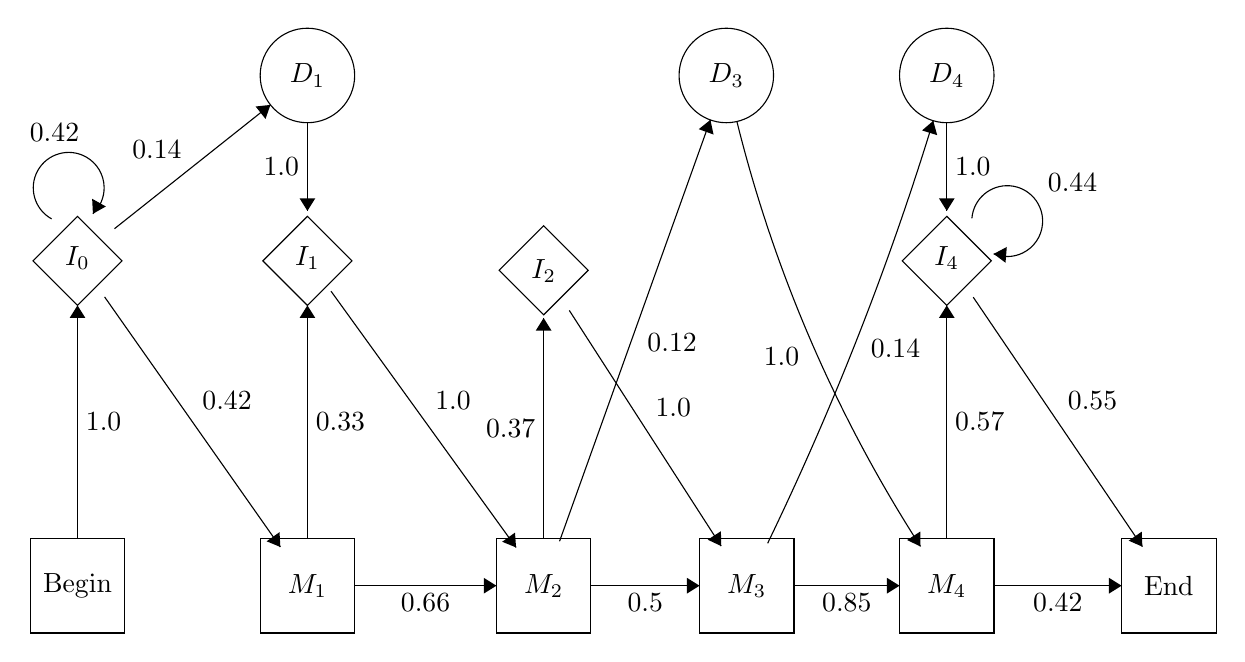
\begin{tikzpicture}[scale=0.2]
\tikzstyle{every node}+=[inner sep=0pt]
\draw [black] (1.9,-45.2) rectangle ++(6,6);
\draw (4.9,-42.2) node {Begin};
\draw [black] (71.2,-45.2) rectangle ++(6,6);
\draw (74.2,-42.2) node {End};
\draw [black] (16.5,-45.2) rectangle ++(6,6);
\draw (19.5,-42.2) node {$M_1$};
\draw [black] (31.5,-45.2) rectangle ++(6,6);
\draw (34.5,-42.2) node {$M_2$};
\draw [black] (44.4,-45.2) rectangle ++(6,6);
\draw (47.4,-42.2) node {$M_3$};
\draw [black] (57.1,-45.2) rectangle ++(6,6);
\draw (60.1,-42.2) node {$M_4$};
\draw [black,rotate around={45:(4.9,-24.4)}] (4.9,-24.4) rectangle ++(4,4);
\draw (4.9,-21.4) node {$I_0$};
\draw [black, rotate around={45:(19.5,-24.4)}] (19.5,-24.4) rectangle ++(4,4);
\draw (19.5,-21.4) node {$I_1$};
\draw [black,rotate around={45:(34.5,-25)}] (34.5,-25) rectangle ++(4,4);
\draw (34.5,-22.2) node {$I_2$};
\draw [black,rotate around={45:(60.1,-24.4)}] (60.1,-24.4) rectangle ++(4,4);
\draw (60.1,-21.4) node {$I_4$};
\draw [black] (19.5,-9.8) circle (3);
\draw (19.5,-9.8) node {$D_1$};
\draw [black] (46.1,-9.8) circle (3);
\draw (46.1,-9.8) node {$D_3$};
\draw [black] (60.1,-9.8) circle (3);
\draw (60.1,-9.8) node {$D_4$};
\draw [black] (22.5,-42.2) -- (31.5,-42.2);
\fill [black] (31.5,-42.2) -- (30.7,-41.7) -- (30.7,-42.7);
\draw (27,-42.7) node [below] {$0.66$};
\draw [black] (37.5,-42.2) -- (44.4,-42.2);
\fill [black] (44.4,-42.2) -- (43.6,-41.7) -- (43.6,-42.7);
\draw (40.95,-42.7) node [below] {$0.5$};
\draw [black] (50.4,-42.2) -- (57.1,-42.2);
\fill [black] (57.1,-42.2) -- (56.3,-41.7) -- (56.3,-42.7);
\draw (53.75,-42.7) node [below] {$0.85$};
\draw [black] (63.1,-42.2) -- (71.2,-42.2);
\fill [black] (71.2,-42.2) -- (70.4,-41.7) -- (70.4,-42.7);
\draw (67.15,-42.7) node [below] {$0.42$};
\draw [black] (3.255,-18.905) arc (241.12502:-46.87498:2.25);
\draw (3.44,-14) node [above] {$0.42$};
\fill [black] (5.88,-18.58) -- (6.7,-18.12) -- (5.83,-17.63);
\draw [black] (4.9,-39.2) -- (4.9,-24.4);
\fill [black] (4.9,-24.4) -- (4.4,-25.2) -- (5.4,-25.2);
\draw (5.4,-31.8) node [right] {$1.0$};
\draw [black] (7.25,-19.53) -- (17.15,-11.67);
\fill [black] (17.15,-11.67) -- (16.21,-11.77) -- (16.84,-12.56);
\draw (9.94,-15.1) node [above] {$0.14$};
\draw [black] (19.5,-12.8) -- (19.5,-18.4);
\fill [black] (19.5,-18.4) -- (20,-17.6) -- (19,-17.6);
\draw (19,-15.6) node [left] {$1.0$};
\draw [black] (21,-23.5) -- (32.75,-39.77);
\fill [black] (32.75,-39.77) -- (32.68,-38.83) -- (31.87,-39.41);
\draw (27.59,-30.42) node [right] {$1.0$};
\draw [black] (60.1,-39.2) -- (60.1,-24.4);
\fill [black] (60.1,-24.4) -- (59.6,-25.2) -- (60.6,-25.2);
\draw (60.6,-31.8) node [right] {$0.57$};
\draw [black] (61.78,-23.88) -- (72.52,-39.72);
\fill [black] (72.52,-39.72) -- (72.48,-38.77) -- (71.65,-39.34);
\draw (67.76,-30.46) node [right] {$0.55$};
\draw [black] (6.62,-23.86) -- (17.78,-39.74);
\fill [black] (17.78,-39.74) -- (17.73,-38.8) -- (16.91,-39.38);
\draw (12.8,-30.44) node [right] {$0.42$};
\draw [black] (19.5,-39.2) -- (19.5,-24.4);
\fill [black] (19.5,-24.4) -- (19,-25.2) -- (20,-25.2);
\draw (20,-31.8) node [right] {$0.33$};
\draw [black] (61.694,-18.872) arc (175.49933:-112.50067:2.25);
\draw (66.49,-16.59) node [right] {$0.44$};
\fill [black] (63.08,-21.13) -- (63.83,-21.69) -- (63.91,-20.69);
\draw [black] (34.5,-39.2) -- (34.5,-25.2);
\fill [black] (34.5,-25.2) -- (34,-26) -- (35,-26);
\draw (34,-32.2) node [left] {$0.37$};
\draw [black] (36.13,-24.72) -- (45.77,-39.68);
\fill [black] (45.77,-39.68) -- (45.76,-38.74) -- (44.92,-39.28);
\draw (41.57,-30.89) node [right] {$1.0$};
\draw [black] (35.51,-39.38) -- (45.09,-12.62);
\fill [black] (45.09,-12.62) -- (44.35,-13.21) -- (45.29,-13.55);
\draw (41.06,-26.77) node [right] {$0.12$};
\draw [black] (58.433,-39.706) arc (-147.2053:-166.05647:89.743);
\fill [black] (58.43,-39.71) -- (58.42,-38.76) -- (57.58,-39.3);
\draw (50.76,-27.66) node [left] {$1.0$};
\draw [black] (59.245,-12.675) arc (-17.02408:-25.78383:188.7);
\fill [black] (59.24,-12.68) -- (58.53,-13.29) -- (59.49,-13.59);
\draw (55.25,-27.16) node [right] {$0.14$};
\draw [black] (60.1,-12.8) -- (60.1,-18.4);
\fill [black] (60.1,-18.4) -- (60.6,-17.6) -- (59.6,-17.6);
\draw (60.6,-15.6) node [right] {$1.0$};
\end{tikzpicture}
\end{center}
$\pi_{Begin}=1.0$ and $\pi$ for all other states is $0.0$. \\
The following table shows the emission probabilities.
\begin{table}[H]
    \centering
    \begin{tabular}{|c|c|c|c|c|}
    \hline
        & $\omega_A$ & $\omega_C$ & $\omega_G$ & $\omega_T$ \\\hline
         $M_1$&  0.16 & 0.83 & 0.0 & 0.0\\\hline
         $M_2$& 0.0 & 0.0 & 0.13 & 0.88\\\hline
         $M_3$& 0.0 & 0.86 & 0.14 & 0.0\\\hline
         $M_4$& 0.71 & 0.0 & 0.0 & 0.29\\\hline
         $I_0$& 0.25 &0.25 &0.25 &0.25 \\\hline
         $I_1$& 0.25 &0.25 &0.25 &0.25\\\hline
         $I_2$& 0.25 &0.25 &0.25 &0.25\\\hline
         $I_3$& 0.25 &0.25 &0.25 &0.25\\\hline
         $I_4$& 0.25 &0.25 &0.25 &0.25 \\\hline
    \end{tabular}
    \caption{Emission Probabilities}
\end{table}
Delete states and Begin-End states do not emit any symbols.
\newpage

The table below also shows the transition probabilities as a table. Note that each row sums up to $1$ except for the End state.
\begin{table}[H]
\begin{tabular}{|l|l|l|l|l|l|l|l|l|l|l|l|l|l|}
\hline
      & Begin & $M_1$            & $M_2$            & $M_3$           & $M_4$           & $I_0$            & $I_1$            & $I_2$            & $I_4$            & $D_1$            & $D_3$            & $D_4$            & End           \\ \hline
Begin & 0.0   & 0.0           & 0.0           & 0.0          & 0.0           & \textbf{1.0}  & 0.0           & 0.0           & 0.0           & 0.0           & 0.0           & 0.0           & 0.0           \\ \hline
$M_1$    & 0.0   & 0.0           & \textbf{0.66} & 0.0          & 0.0           & 0.0           & \textbf{0.33} & 0.0           & 0.0           & 0.0           & 0.0           & 0.0           & 0.0           \\ \hline
$M_2$    & 0.0   & 0.0           & 0.0           & \textbf{0.5} & 0.0           & 0.0           & 0.0           & \textbf{0.37} & 0.0           & 0.0           & \textbf{0.12} & 0.0           & 0.0           \\ \hline
$M_3$    & 0.0   & 0.0           & 0.0           & 0.0          & \textbf{0.85} & 0.0           & 0.0           & 0.0           & 0.0           & 0.0           & 0.0           & \textbf{0.14} & 0.0           \\ \hline
$M_4$    & 0.0   & 0.0           & 0.0           & 0.0          & 0.0           & 0.0           & 0.0           & 0.0           & \textbf{0.57} & 0.0           & 0.0           & 0.0           & \textbf{0.42} \\ \hline
$I_0$    & 0.0   & \textbf{0.42} & 0.0           & 0.0          & 0.0           & \textbf{0.42} & 0.0           & 0.0           & 0.0           & \textbf{0.14} & 0.0           & 0.0           & 0.0           \\ \hline
$I_1$    & 0.0   & 0.0           & \textbf{1.0}           & 0.0          & 0.0           & 0.0           & 0.0           & 0.0           & 0.0           & 0.0           & 0.0           & 0.0           & 0.0           \\ \hline
$I_2$    & 0.0   & 0.0           & 0.0           & \textbf{1.0}          & 0.0           & 0.0           & 0.0           & 0.0           & 0.0           & 0.0           & 0.0           & 0.0           & 0.0           \\ \hline
$I_4$    & 0.0   & 0.0           & 0.0           & 0.0          & 0.0           & 0.0           & 0.0           & 0.0           & \textbf{0.44} & 0.0           & 0.0           & 0.0           & \textbf{0.55} \\ \hline
$D_1$    & 0.0   & 0.0           & 0.0           & 0.0          & 0.0           & 0.0           & \textbf{1.0}  & 0.0           & 0.0           & 0.0           & 0.0           & 0.0           & 0.0           \\ \hline
$D_3$    & 0.0   & 0.0           & 0.0           & 0.0          & \textbf{1.0}  & 0.0           & 0.0           & 0.0           & 0.0           & 0.0           & 0.0           & 0.0           & 0.0           \\ \hline
$D_4$    & 0.0   & 0.0           & 0.0           & 0.0          & 0.0           & 0.0           & 0.0           & 0.0           & \textbf{1.0}  & 0.0           & 0.0           & 0.0           & 0.0           \\ \hline
End   & 0.0   & 0.0           & 0.0           & 0.0          & 0.0           & 0.0           & 0.0           & 0.0           & 0.0           & 0.0           & 0.0           & 0.0           & 0.0           \\ \hline
\end{tabular}
\caption{Transition Probabilities}
\end{table}
\newpage
\section*{Part B}
\begin{table}[H]
\resizebox{\columnwidth}{!}{\begin{tabular}{|c|c|c|c|c|c|c|c|c|c|c|c|c|c|}
\hline
\textbf{}   & Begin & $I_0$    & $M_1$    & $I_1$    & $D_1$    & $M_2$    & $I_2$    & $M_3$    & $D_3$    & $M_4$    & $I_4$   & $D_4$    & End \\ \hline
\textbf{""} & 1.0   & 0.0     & 0.0     & 0.0     & 0.0     & 0.0     & 0.0     & 0.0     & 0.0     & 0.0     & 0.0    & 0.0     & 0.0 \\ \hline
\textbf{C}  & 0.0   & 0.25    & 0.0     & 0.0     & 3.57e-2     & 0.0     & 0.0     & 0.0     & 0.0     & 0.0     & 0.0    & 0.0     & 0.0 \\ \hline
\textbf{T}  & 0.0   & 2.62e-2 & 0.0     & 8.93e-3     & 3.67e-3 & 0.0     & 0.0     & 0.0     & 0.0     & 0.0     & 0.0    & 0.0     & 0.0 \\ \hline
\textbf{C}  & 0.0   & 2.75e-3 & 9.13e-3 & 9.18e-4 & 3.85e-4 & 0.0     & 0.0     & 0.0     & 0.0     & 0.0     & 0.0    & 0.0     & 0.0 \\ \hline
\textbf{T}  & 0.0   & 2.89e-4 & 0.0     & 7.53e-4 & 4.05e-5 & 5.3e-3  & 0.0     & 0.0     & 6.36e-4 & 0.0     & 0.0    & 0.0     & 0.0 \\ \hline
\textbf{G}  & 0.0   & 3.03e-5 & 0.0     & 1.01e-5 & 4.24e-6 & 9.79e-5 & 4.9e-4  & 3.71e-4 & 1.17e-5 & 0.0     & 0.0    & 5.19e-5 & 0.0 \\ \hline
\textbf{A}  & 0.0   & 3.18e-6 & 2.04e-6 & 1.06e-6 & 4.45e-7 & 0.0     & 9.06e-6 & 0.0     & 0.0     & 2.24e-4 & 1.3e-5 & 0.0     & 9.4e-5 \\ \hline
\end{tabular}}
\caption{Partial Probability Table}
\end{table}
If we trace back the table that we filled using \textit{Viterbi Algorithm}, we get the following sequence of states:
\[
\text{Begin} \rightarrow I_0 \rightarrow I_0 \rightarrow M_1 \rightarrow M_2 \rightarrow M_3 \rightarrow M_4 \rightarrow \text{End}
\]
According to the table, we end up in $M_4$ state with $2.24e-4$ probability and since we go to \textit{End} state with $0.42$ probability, we get $2.24e-4\times 0.42=9.4e-5$.
\end{document}
